\begin{frame}{Nachbearbeitung in GeoMagic}

\begin{block}{Nachbearbeitungsschritte}
\begin{enumerate}
\item Registrierung
\begin{enumerate}
\item Globale Registrierung in Gruppen
\item Manuelle Registrierung der Gruppen, n-Punkt Registrierung
\end{enumerate}
\item Meshgenerierung
\begin{enumerate}
\item Vereinigen der registrierten Meshes
\end{enumerate}
\item Nachbearbeitung
\begin{enumerate}
\item Nachbearbeitung: 2D-Mannigkeitsfehler entfernen, Glätten, Spitzen entfernen, Mesh-Doctor, Löcher füllen
\item Feine Nachbearbeitung: Sandpapier
\end{enumerate}
\end{enumerate}
\end{block}

\end{frame}

\begin{frame}{Registrierung}

\begin{block}{globale Registrierung}
\begin{figure}[H]
\centering
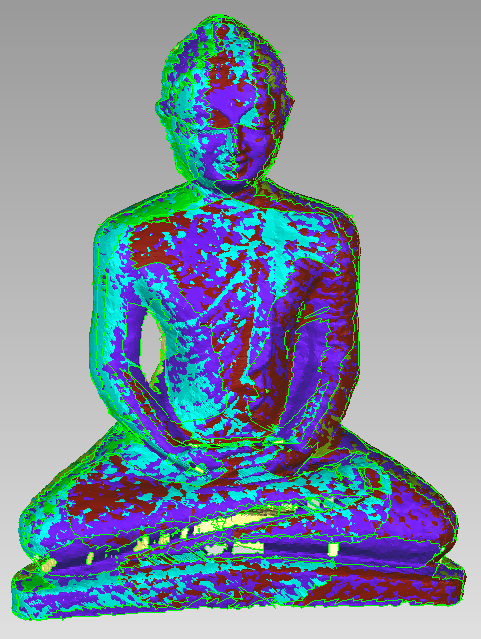
\includegraphics[width=0.4\textwidth]{images/GeoMagicBudhaPictures/Budha_Scans_Aufrecht_globalRegistration_2.PNG}
\caption{Globale Registrierung - Falschfarbendarstellung verschiedener Range Maps}
\label{fig:budhaGlobal}
\end{figure}
\end{block}

\end{frame}

\begin{frame}{Registrierung}

\begin{block}{manuelle n-Punkt Registrierung}
\begin{figure}[H]
\centering
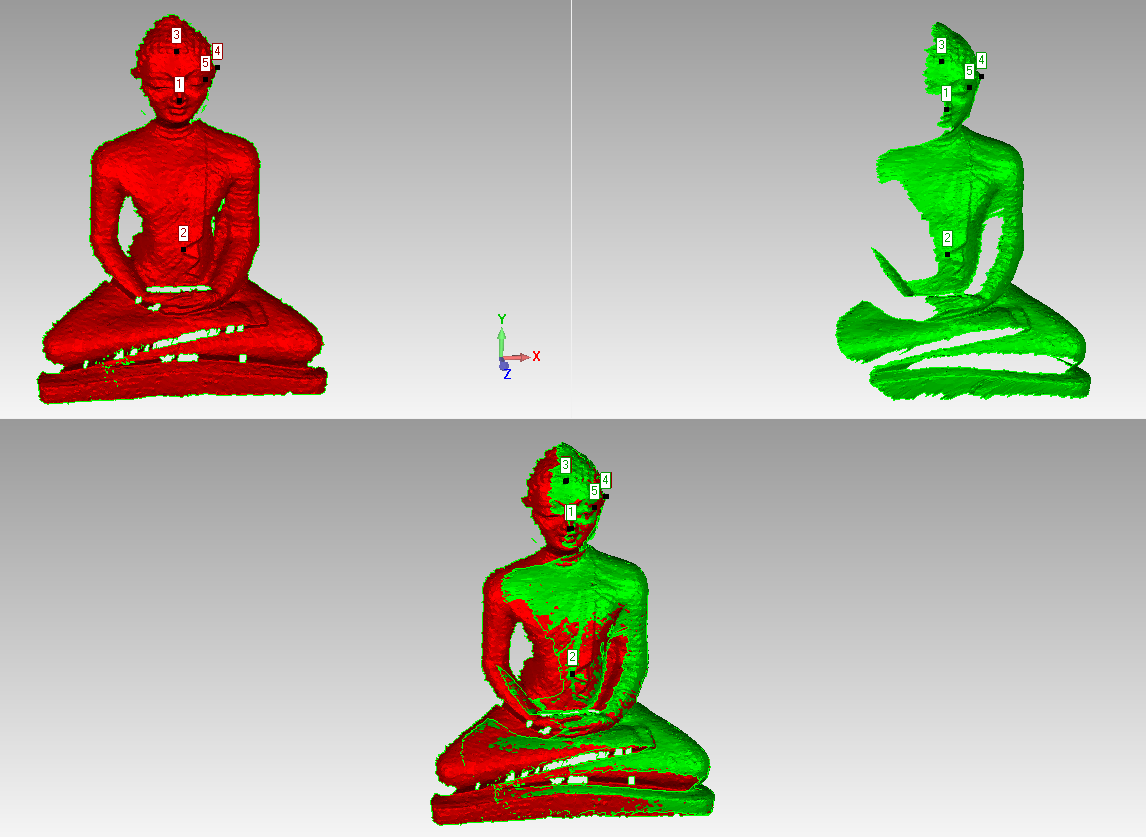
\includegraphics[width=0.65\textwidth]{images/GeoMagicBudhaPictures/Budha_Scans_Aufrecht_manualRegistration_03.PNG}
\caption{Manuelle Registrierung mittels verteilter Punkte}
\label{fig:budhaManual}
\end{figure}
\end{block}

\end{frame}


\begin{frame}{Meshverarbeitung}

\begin{block}{Mesh Doctor}
\begin{figure}[H]
\centering
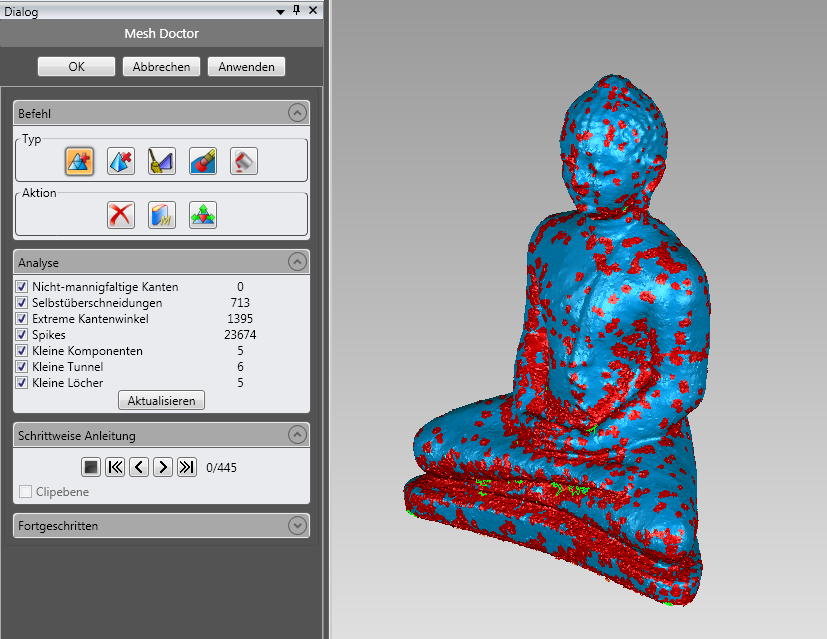
\includegraphics[width=0.5\textwidth]{images/GeoMagicBudhaPictures/Budha_MeshDoctor.PNG}
\caption{Mesh-Doktor - Highlighting von defekten oder zu bearbeitenden Stellen}
\label{fig:budhaMeshDoc}
\end{figure}
\end{block}

\end{frame}

\begin{frame}{Meshverarbeitung}

\begin{block}{Löcher schließen}
\begin{table}[h]
	\begin{center}
		\begin{tabular}{| c | c |}
			\hline
			offen & geschlossen \\
			\hline
			\hline
			& \\
			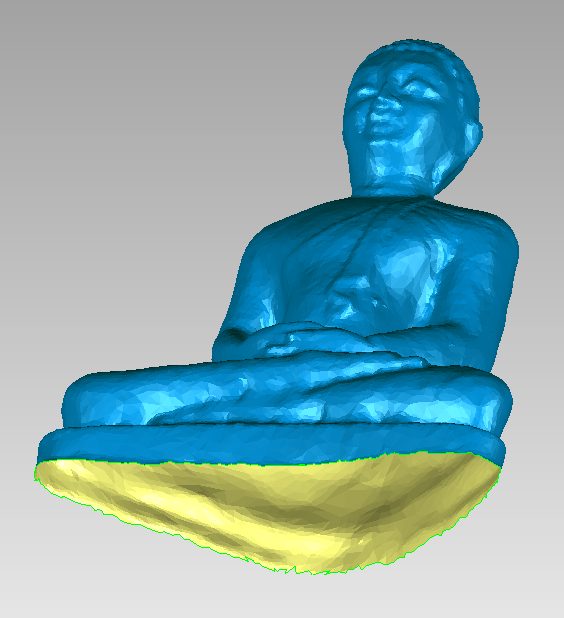
\includegraphics[width=0.35\textwidth]{./Images/GeomagicBudhaPictures/Budha_SfM_BottomHole_2.PNG} & 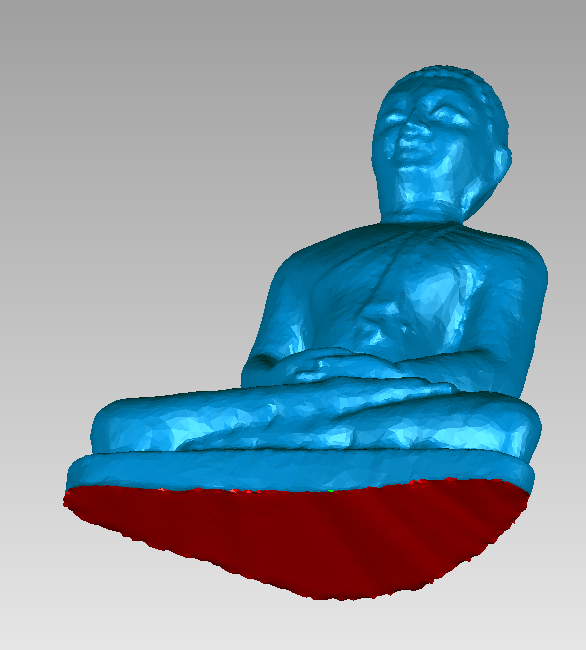
\includegraphics[width=0.345\textwidth]{./Images/GeomagicBudhaPictures/Budha_SfM_BottomHoleClosed_2.PNG} \\
			\hline					  
		\end{tabular}
	\end{center}
	\caption{Manuelles Schließen der Grundfläche einer Figur, links vorher, rechts nachher}
	\label{tab:BudhaHole}
\end{table}
\end{block}

\end{frame}

\begin{frame}{Meshverarbeitung}

\begin{block}{Glätten}
\begin{table}[h]
	\begin{center}
		\begin{tabular}{| c | c |}
			\hline
			vor Glättung & nach Glättung \\
			\hline
			\hline
			& \\
			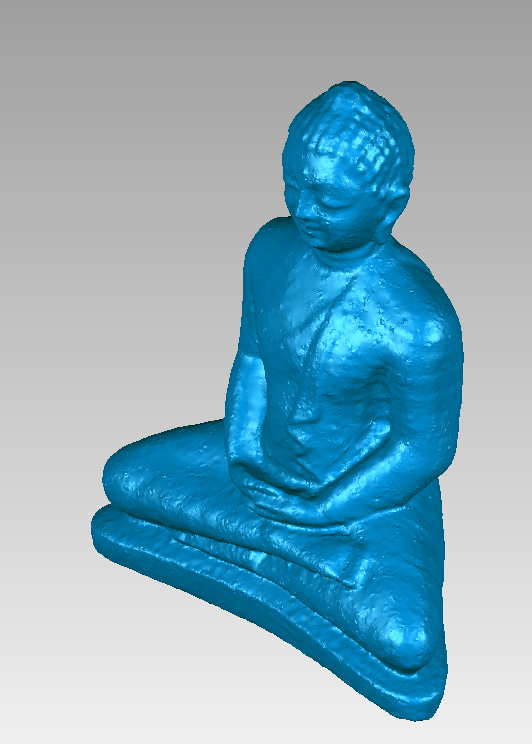
\includegraphics[width=0.30\textwidth]{./Images/GeomagicBudhaPictures/Budha_Presmooth.PNG} & 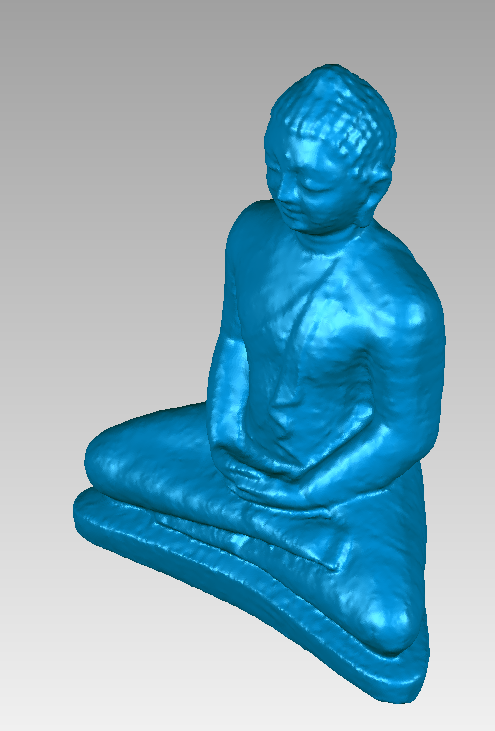
\includegraphics[width=0.285\textwidth]{./Images/GeomagicBudhaPictures/Budha_Postsmooth.PNG} \\
			\hline					  
		\end{tabular}
	\end{center}
	\caption{Manuelles Glätten einer Figur, links vorher, rechts nachher}
	\label{tab:BudhaSmooth}
\end{table}
\end{block}

\end{frame}